\section{Tape-Out}
\label{sec:tapout}
Our initial objective was to conclude the chip design phase of this project within the scope of our first project thesis. However, unexpected delays in our timeline led to us missing the initial tape-out deadline. A substantial portion of this delay stemmed from the necessity to overhaul the buck-boost converter regulator loop. We were compelled to transition from the previously implemented average current-mode control to peak current-mode control due to certain encountered issues. Despite the provision of an extended timeline, finalizing the design before the deadline remained a challenging task. This time pressure resulted in us hastening certain aspects of the design and eliminating nonessential features, such as the over-temperature protection circuit we had initially designed.

\subsection{Buck-Boost Converter}
The layout of the buck-boost converter can be seen in  \autoref{fig:BBlayout} with annotations showing the rough floorplan of the circuit. Surrounding the converter are the four large switching transistors which increased significantly in size between initial planning in the previous thesis and to what we ultimately implemented. The exact values and sizes are listed in \autoref{tab:spec_pmos} and \autoref{tab:spec_nmos}. The largest contributor to the losses in the power-stage surprisingly are the metal trace resistances which increased the theoretical $R_{DS,on}$ of the \ac{PMOS} transistors from \qty{58.3}{\milli\ohm} to an effective value of \qty{240}{\milli\ohm} in post-layout simulations. These metal resistances could not be further minimized through wider traces as the limiting factor was the maximum metal density for manufacturing. \\
The large empty space above the error amplifier in \autoref{fig:BBlayout} was initially intended for a temperature sensing circuit in order to measure the rough temperature of the power electronics and to disable operation in case of an over temperature event. Due to the tight timeline we opted not to layout this circuit as we were already significantly behind schedule and needed the time to finish the layout of other critical circuits. Due to the same reason we implemented only the bare-minimum of \ac{DFT} functionality to measure the oscillator clock frequency, the bandgap reference voltage and the internal current reference. As a result the rest of the chip is with respect to troubleshooting a black-box with no possibility to measure internal signals.

\begin{table}[H]
    \centering
    \begin{tabular}{|c|c|c|}
        Characteristic & Planned Value & Implemented Value \\
        \hline
		 Typ. $R_{DS,on}$ & \qty{113}{\milli\ohm}  & \qty{58.3}{\milli\ohm} \\
         \# of Transistors & \qty{4834}{}  & \qty{9408}{} \\
		 Width & \qty{96.7}{\milli\meter} & \qty{188.2}{\milli\meter}\\
		 Size & \qty{1000.2}{\micro\meter} x \qty{486.8}{\micro\meter} & \qty{1228.8}{\micro\meter} x \qty{764.4}{\micro\meter}
    \end{tabular}
    \caption{Specifications of the power \ac{PMOS}}
    \label{tab:spec_pmos}
\end{table}

\begin{table}[H]
    \centering
    \begin{tabular}{|c|c|c|}
        Characteristic & Planned Value & Implemented Value \\
        \hline
		 Typ. $R_{DS,on}$ & \qty{72.8}{\milli\ohm} & \qty{37}{\milli\ohm} \\
         \# of Transistors & \qty{2800}{}  & \qty{6080}{} \\
		 Width & \qty{56}{\milli\meter} & \qty{121.6}{\milli\meter} \\
		 Size & \qty{641.4}{\micro\meter} x \qty{483.1}{\micro\meter} & \qty{972.8}{\micro\meter} x \qty{688}{\micro\meter}
    \end{tabular}
    \caption{Specifications of the power \ac{NMOS}}
    \label{tab:spec_nmos}
\end{table}

\begin{figure}[h]
    \centering
    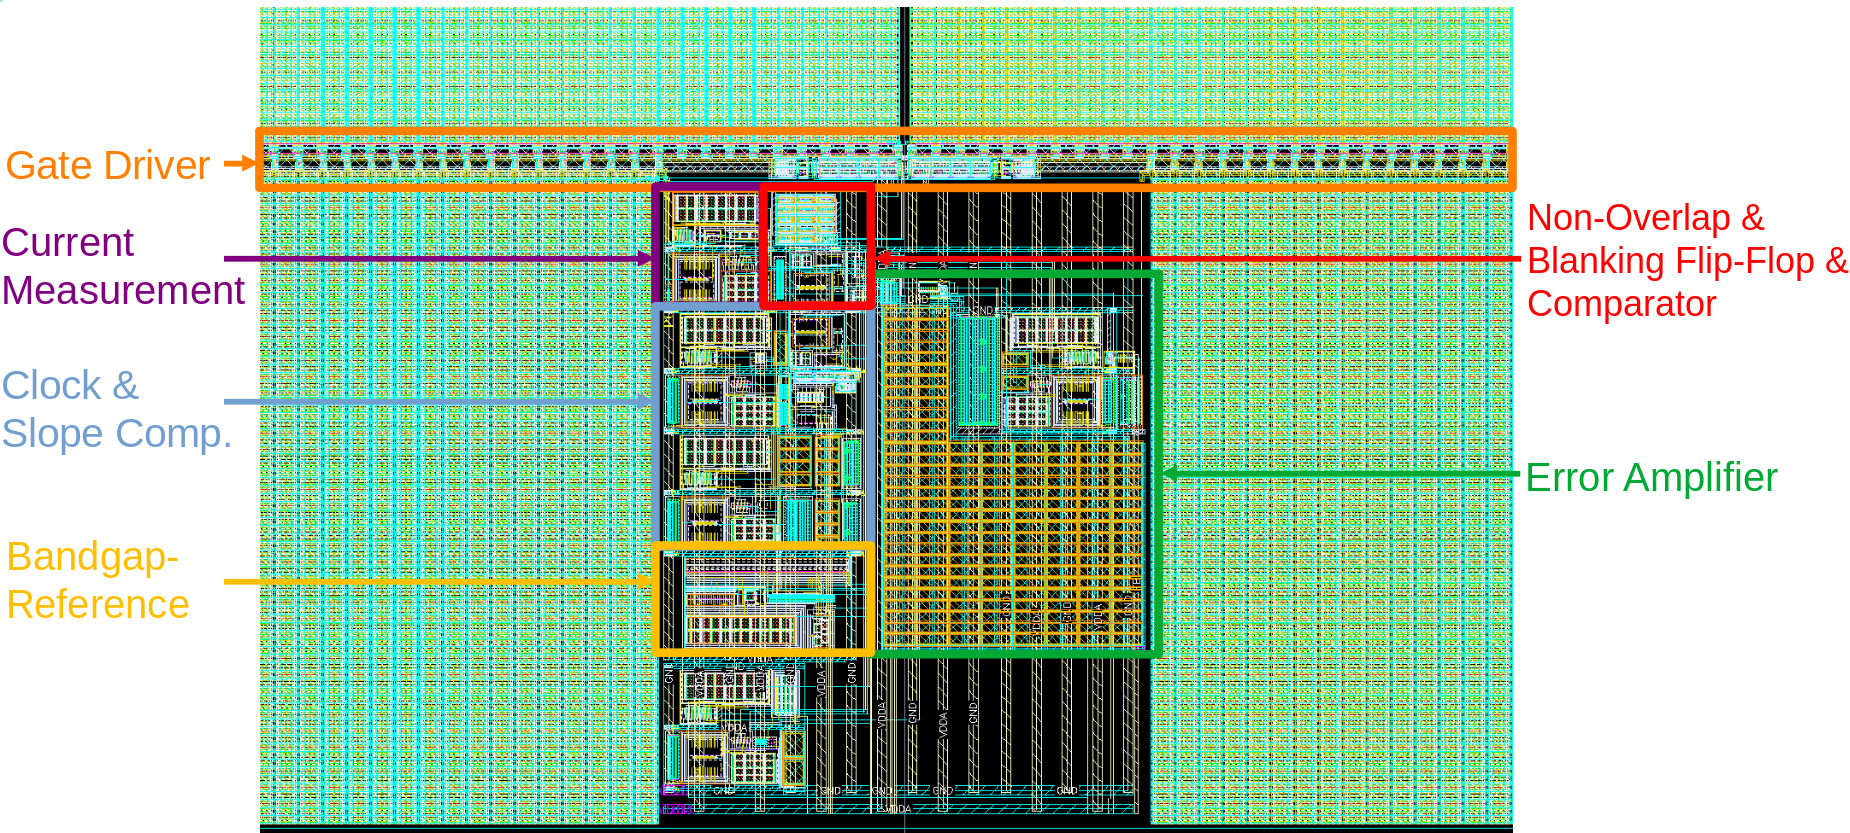
\includegraphics[width=1\textwidth]{../ASIC-DESIGN-2/images/07_DCDC/BuckBoostLayout.png}
    \caption{Layout of the buck-boost converter regulator surrounded by the large power stage transistors}
    \label{fig:BBlayout}
\end{figure}

\clearpage

\subsection{Overall Chip Floorplan}
As can be seen in \autoref{fig:chiplayout}, this design is significantly pad limited as opposed to core limited. The entire lower right corner is unused and in general the lower third is sparsely populated. Conversely the upper two thirds which is entirely filled the the buck-boost converter. The large switching transistors were maximized in size to reduce conversions losses and take up the majority of the chips area. A large number of pads are used in parallel for the converters input, output and switching nodes to meet our current handling capabilities and not exceed the recommendation of \qty{50}{\milli\ampere} per pad. In the bottom left the digital circuitry for the \ac{SPI} periphery and internal registers can be seen as well as supporting circuitry like the \ac{POR} and bandgap voltage reference. 
\begin{table}[H]
    \centering
    \begin{tabular}{|c|c|}
        Property & Value \\
        \hline
        Function & Buck-Boost Converter \\
        Package & QFN48 7x\qty{7}{\milli\meter} \\
        Process & X-FAB \qty{350}{\nano\meter} \\
		Size & \qty{2712}{\micro\meter} x \qty{2952}{\micro\meter} \\
        Area & \qty{8.006}{\milli\meter\squared}
    \end{tabular}
    \caption{ASIC Properties}
    \label{tab:spec_asic}
\end{table}
\begin{figure}[h]
    \centering
    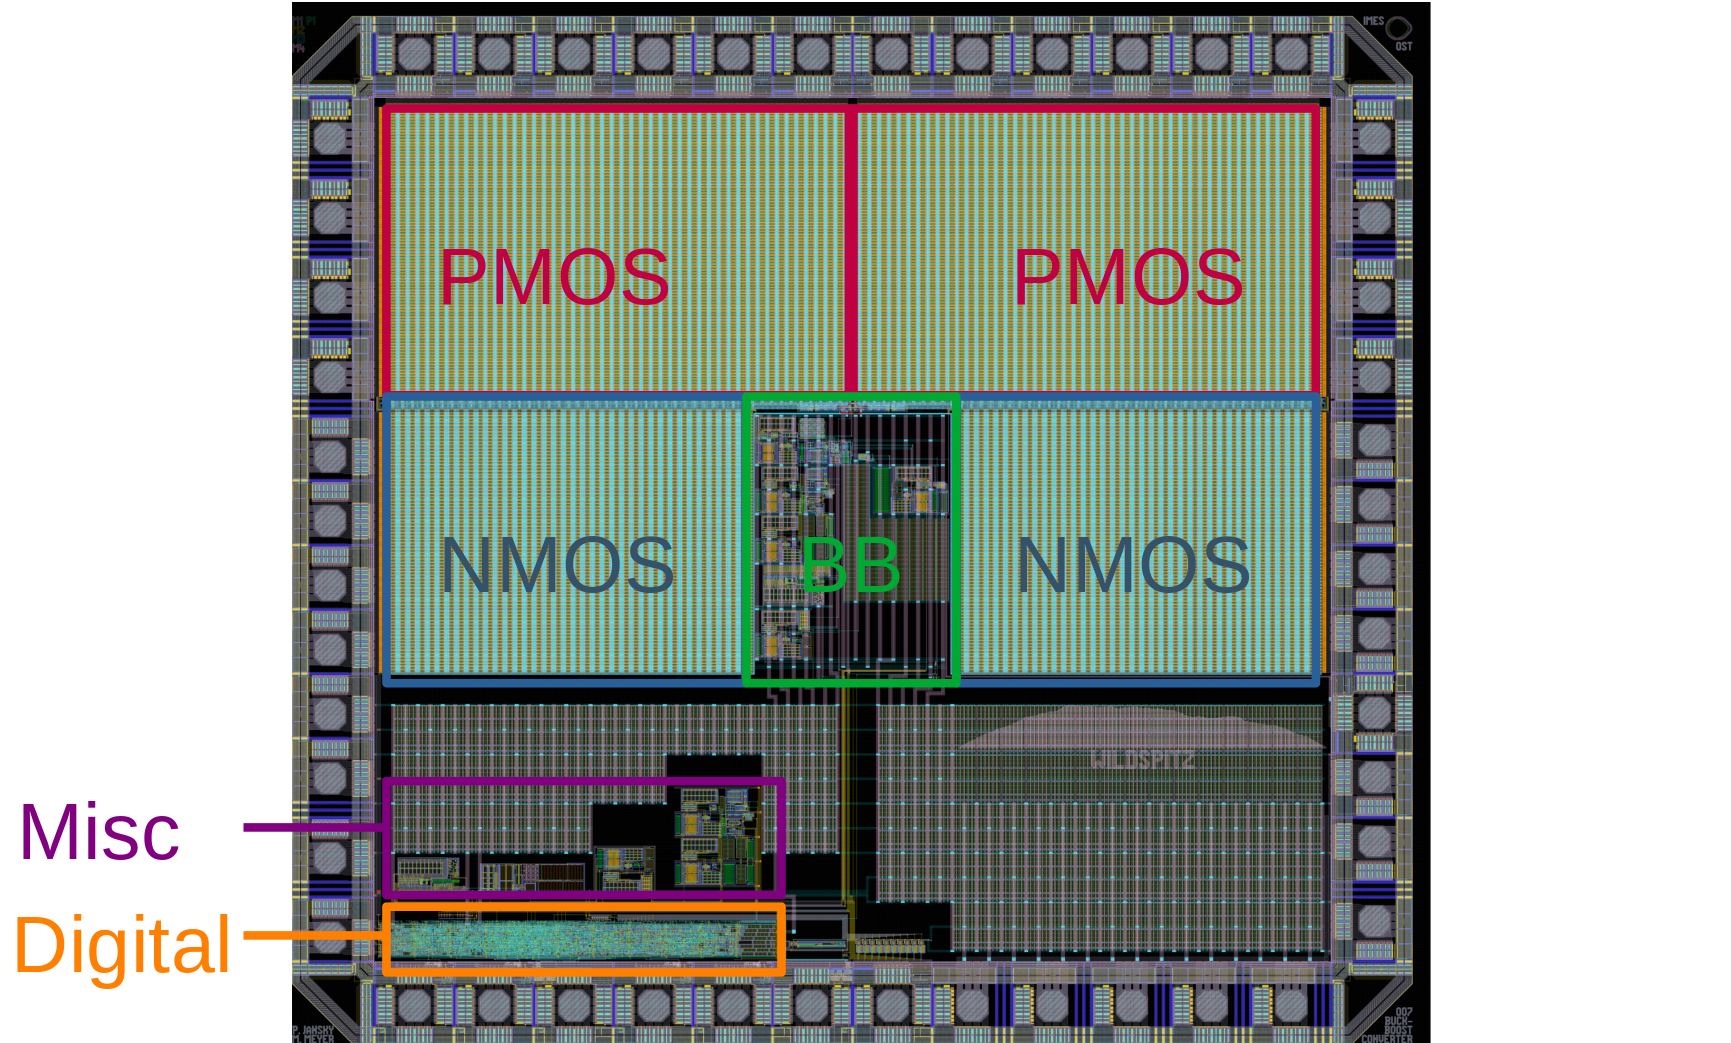
\includegraphics[width=1\textwidth]{../ASIC-DESIGN-2/images/07_DCDC/ChipLayout.png}
    \caption{Floorplan of the entire chip with annotations}
    \label{fig:chiplayout}
\end{figure}
\subsubsection{Package}
In \autoref{fig:package}, the package (QFN-48) of the chip is illustrated. It is evident that there are two distinct ground connections, namely GND and GND\_2, and two separate supply voltages, V\_IN and VDD\_D. These two domains can be interconnected on the \ac{PCB}. However, to minimize noise interference and to facilitate separate analysis of the DC/DC converter and the rest of the circuit, these domains are not internally connected within the chip. Specifically, GND\_2 serves as the ground for the DC/DC converter, while GND is the ground for the digital part, bandgap, current reference, and so on. Similarly, V\_IN is the supply voltage for the DC/DC converter, and VDD\_D is the supply voltage for the remaining circuit components. An exact explanation of all the pins can be found below:
\begin{itemize}
	\item \textbf{A\_OUT:} Analog test point can mux out internal signals. See also \autoref{subsec:spi_interface}.
	\item \textbf{D\_OUT:} Outputs clock when enabled. See also \autoref{subsec:spi_interface}.
	\item \textbf{FB:} Feedback to overwrite output voltage by external voltage divider. (\textcolor{red}{*insert formula here*}).
	\item \textbf{GND:} Ground of Digital logic and reference circuits like Bandgap.
	\item \textbf{GND\_2:} Ground pins for DC/DC converter.
	\item \textbf{L\_IN/L\_OUT:} Connection to external DC/DC coil. (\textcolor{red}{\qty{50}{\milli\henry}}).
	\item \textbf{RST:} Pull to high when you want to reset the chip. Resets the whole chip including the register content of the digital part.
	\item \textbf{SPI*:} SPI interface connections.
	\item \textbf{VDD\_D:} Supply voltage of Digital logic and reference circuits like Bandgap.
	\item \textbf{V\_OUT:} Charging pin of HIs, outputs 5V independent of input voltage (4.3-5.5V, up to 300mA tested).
\end{itemize}
\begin{figure}[h]
	\centering
	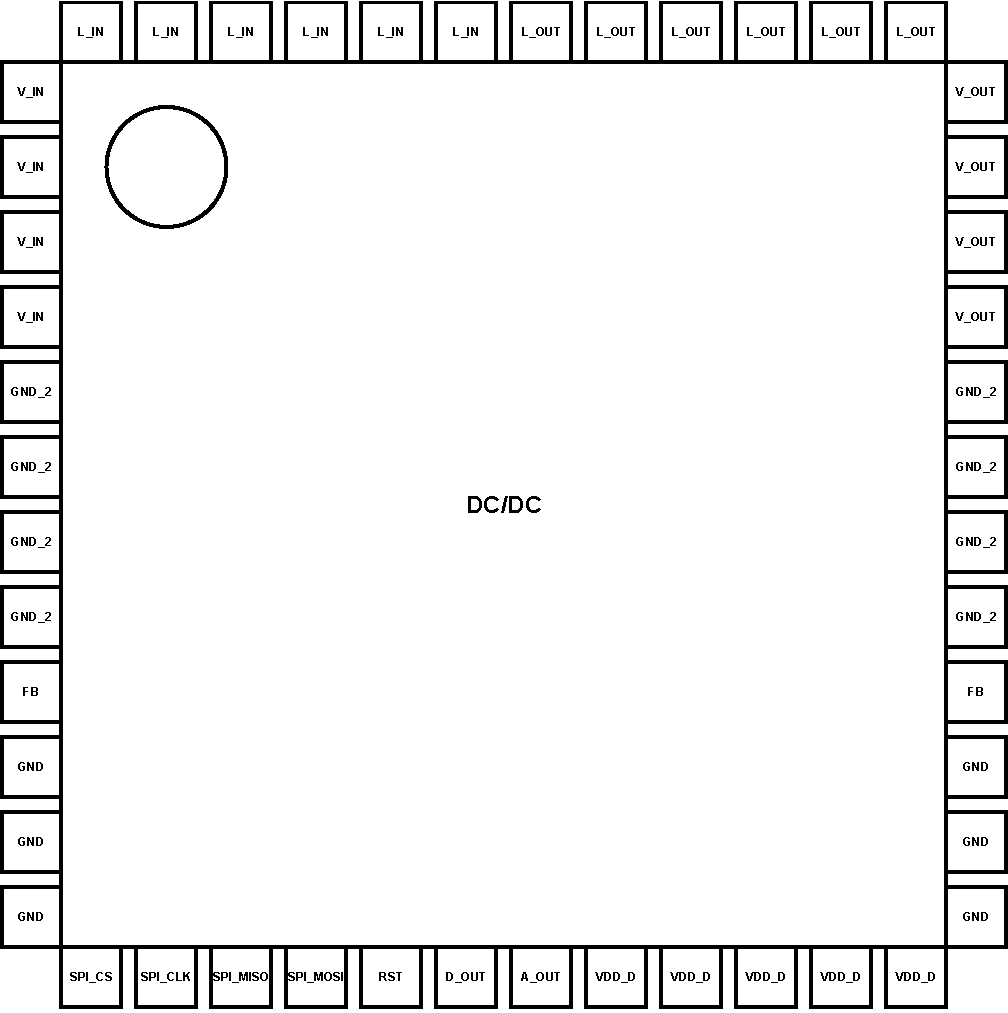
\includegraphics[width=1\textwidth]{../ASIC-DESIGN-2/images/pakage.pdf}
	\caption{Floor-plan Package, Top view}
	\label{fig:package}
\end{figure}
